
\section{Introduction}
In recent years, large language models (LLMs) have garnered significant academic and industrial attention \citep{browngpt3_2020,touvron2023llama}. The scaling law suggests that the validation loss of language models follow a power-law pattern as model and data sizes increase~\citep{hestness2017deep,kaplan2020scaling,henighan2020scaling}. This law provides a powerful framework for forecasting LLM performances before large scale training by fitting losses at smaller scales \citep{achiam2023gpt,deepseek-ai2024deepseek,dubey2024llama}. Numerous studies have explored on the formulation to model the scaling effect of LLMs under various different settings~\citep{bahri2021explaining,hernandez2021scaling,caballero2022broken,Quantization-scaling,muennighoff2023scaling}.

However, typical scaling law formulations focus only on the final loss at the end of training~\citep{hoffmann2022training}. Specifically, previous approaches generally rely on a set of training runs and fit the scaling law curve solely on the final loss from each run. Essentially, the middle points with different degrees of LR annealing fail to follow typical scaling laws, which do not consider local loss drop brought by LR annealing. 
The previous approach under-utilizes the training compute and fails to capture the \emph{training dynamics} within each run. Further, the application of scaling laws in LLM developments is limited since the loss curve through the whole training process is not modeled. An expressive formulation that models full loss curves enables prediction of future training dynamics and also offers insights on understanding the learning process of LLMs.
%In other words, the data points used for fitting scaling laws and predicting are the losses incurred after the completion of learning rate scheduler (LRS). 
% Essentially, the middle loss points with different LR annealing degrees fail to follow typical scaling laws, which do not consider local loss drop brought by LR annealing.
% Consequently, these laws are unable to fit or predict a full loss curve. Till this work, we do not have an appropriate formulation that accurately describes the dynamics during the training process, which is crucial to deeply understand and improve the training process.

In this study, we propose a scaling law that models the full loss curve within a complete LLM training run. 
Specifically, we dive deeper into the training dynamics during LR annealing, and incorporate a LR annealing factor into the traditional scaling law formula to formulate the process.
This design is motivated by the observed correlation between LRS and loss curves, where loss gradually decreases as we consume more training steps~\footnote{In this paper, we use training steps to quantify the amount of consumed data, as they are typically proportional, with data amount calculated as training steps multiplied by batch size.} and then sharply declines when the LR undergoes significant annealing~\citep{loshchilov2016sgdr,dontdecay,simple-scalable-cpt2024,hu2024minicpm}. 
Fig.~\ref{fig:similarity} depicts how loss curves change over different learning rate schedules.
Overall, we discover that the validation loss of a language model at any step is determined by two factors: the forward area $S_1$ under the LR curve and the degree of LR annealing $S_2$ at that step. Formally, the expectation of loss $L$ at step $s$ of a language model follows::
\begin{equation}
\label{eq:scaling}
\begin{aligned}
L(s) &= L_0 + A\cdot S_1^{-\alpha} - C\cdot S_2, \\
S_1 &= \sum\limits_{i=1}^{s}\eta_i, \\
S_2 &= \sum\limits_{i=1}^{s}\sum\limits_{k=1}^{i}(\eta_{k-1} - \eta_{k})\cdot \lambda^{i-k},
\end{aligned}
\end{equation}
where $\eta_i$ is the learning rate at step $i$, and $\lambda$ is a hyper-parameter representing the decay factor for LR annealing momentum (see Sec.~\ref{sec:theorem} in detail),which typically ranges from $0.99$ to $0.999$. $L_0$, $A$, $C$, $\alpha$ are undetermined positive constants. $S_1$ is also known as the summed learning rate~\citep{kaplan2020scaling}, and $S_2$ represents the LR annealing area. A visualization of $S_1$ and $S_2$ is provided as Fig.~\ref{fig:definition}. 

Eq.~\ref{eq:scaling} describes how loss changes for each step in a full loss curve during training. In Eq.~\ref{eq:scaling}, the term $L_0 + A\cdot S_1^{-\alpha}$ represents a rectified scaling law that captures the expected loss decreases as a power-law function of the number of training steps. The new term $-C\cdot S_2$ accounts for the further loss drop due to learning rate annealing. Remarkably, this simple formulation accurately describes the validation loss at any training step across various LRS and even allows us to predict the loss curve for unseen LRS. For example, we can fit Eq.~\ref{eq:scaling} to the full loss curve of constant and cosine LRS with 20K total steps (Fig.~\ref{fig:fit}), and then predict the full loss curve for various unseen LRS with longer total steps (e.g. 60K) (Fig.~\ref{fig:prediction}).

\begin{figure}[tbp]
\centering
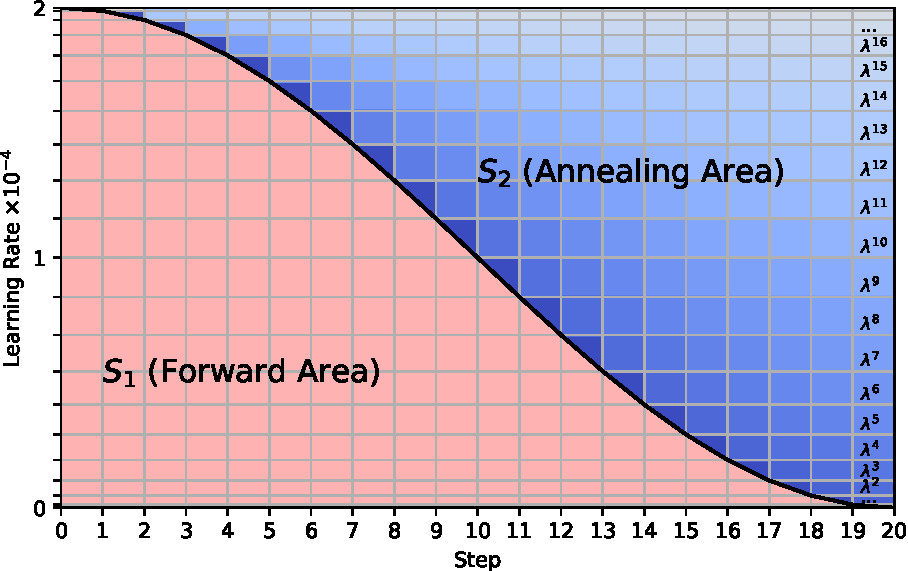
\includegraphics[width=0.8\textwidth]{images/definition}
\caption{Visualization of $S_1$ and $S_2$ at the 20-th step of a cosine LR scheduler. $S_1$ is the forward area, i.e., sum of red grid areas, which can be approximately regarded as the total amount of movement for neural network parameters; $S_2$ is the decayed annealing area, i.e., weighted sum of blue grid areas, where lighter shades indicate smaller weights.
%  (the lighter the color, the greater the degree of decay)
Both $S_1$ and $S_2$ contribute to loss reduction, and balancing their values is crucial for achieving the lowest possible final loss.
}
\label{fig:definition}
\vspace{-10pt}
\end{figure}


% \begin{wrapfigure}{r}{0.5\linewidth}
% \centering
% 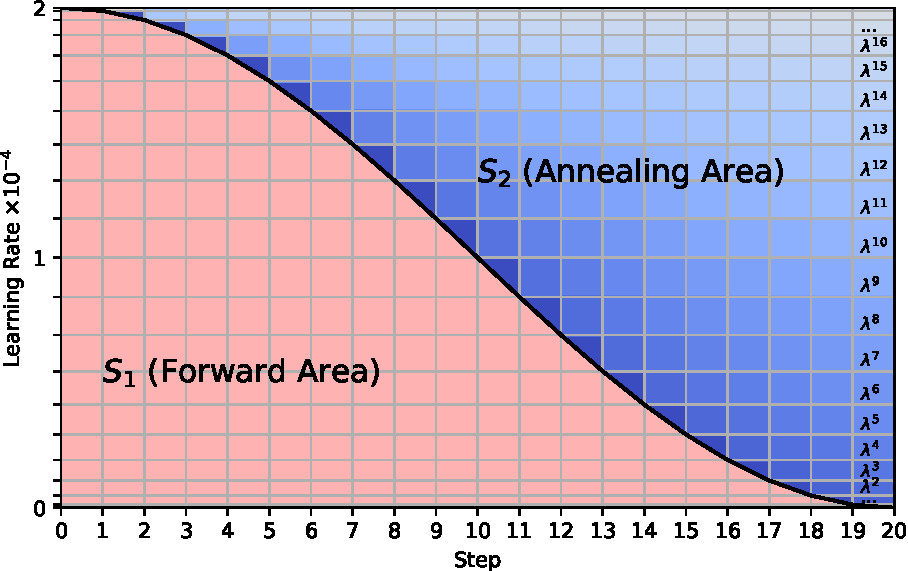
\includegraphics[width=\linewidth]{images/definition}
% \caption{The definition of $S_1$ and $S_2$, taking a 20-step cosine learning rate schedule as a toy example. $S_1$ (forward area) is the area enclosed by the learning rate curve and the X-axis step, which can be approximately regarded as the total amount of movement of neural network parameters; $S_2$ is the decayed annealing area of the learning rate curve (the lighter the color, the greater the degree of decay), that is, the weighted sum of the areas of the small blue squares. 
% %Both the increase of $S_1$ and $S_2$ can help to reduce the loss, but they exist in a delicate balance or trade-off relationship. To minimize the final loss, it's necessary to discover optimal balance between $S_1$ and $S_2$.
% }
% \label{fig:definition}
% \vspace{-10pt}
% \end{wrapfigure}

\begin{figure}[tbp]
    \centering
    \begin{subfigure}[b]{0.32\textwidth}
        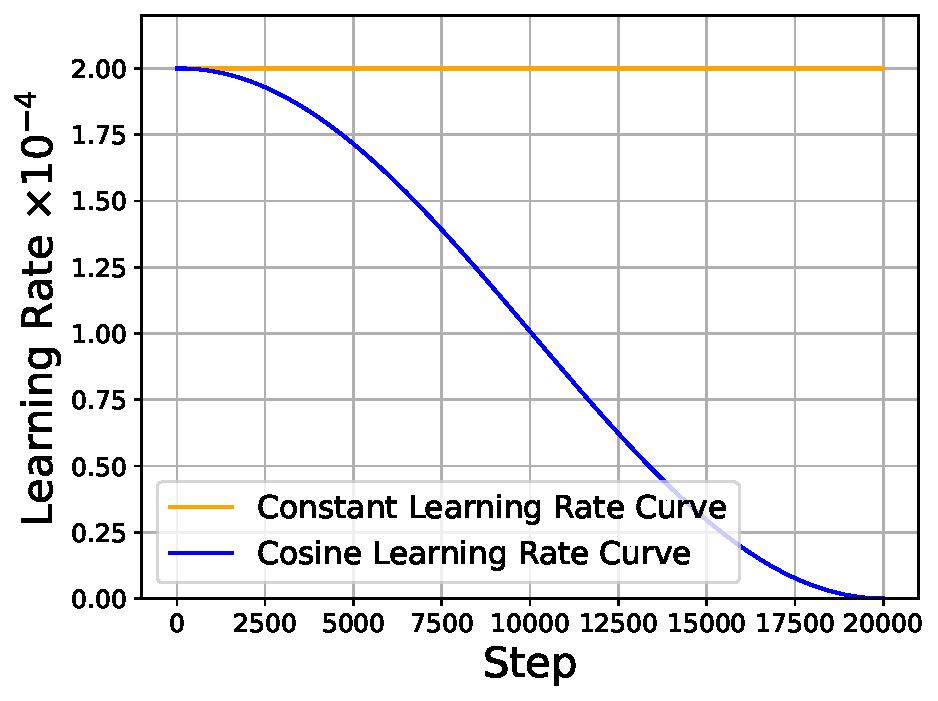
\includegraphics[width=\textwidth]{images/pdfs_0.999_bigbig/lr_constant_and_cosine_2w.pdf}
        \caption{LR curves.}
    \end{subfigure}
    \hfill
    \begin{subfigure}[b]{0.32\textwidth}
        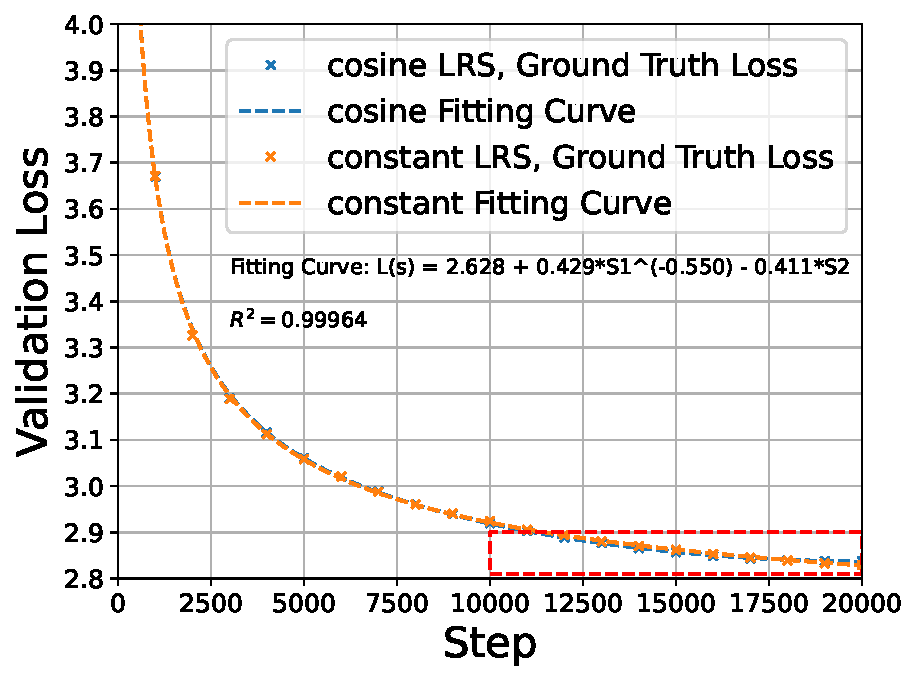
\includegraphics[width=\textwidth]{images/pdfs_0.999_bigbig/fit_0.999_zoomout.pdf}
        \caption{Loss curves.}
    \end{subfigure}
    \hfill
    \begin{subfigure}[b]{0.32\textwidth}
        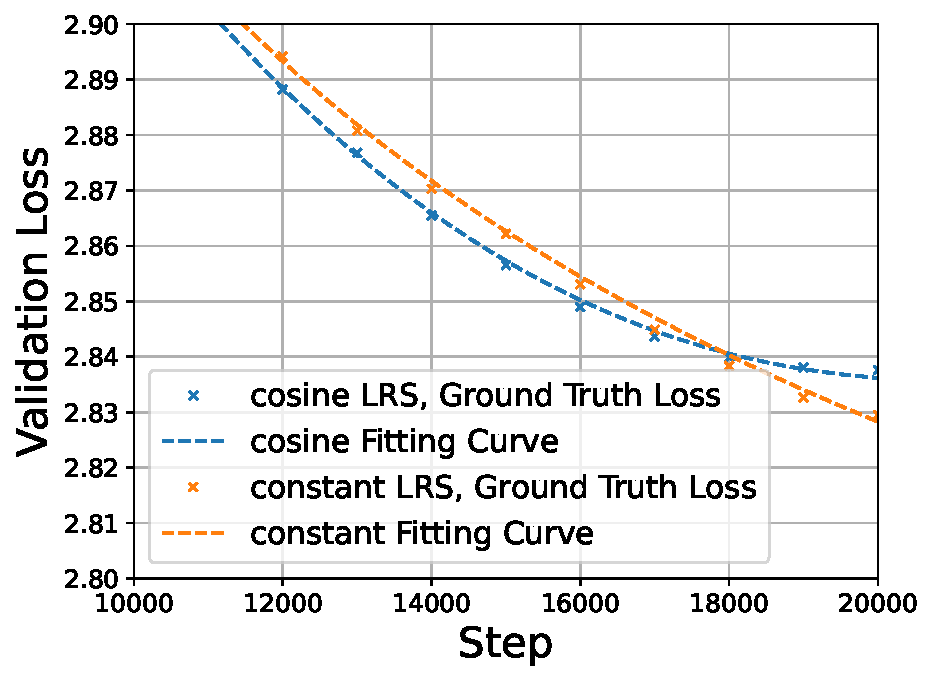
\includegraphics[width=\textwidth]{images/pdfs_0.999_bigbig/fit_0.999_zoomin.pdf}
        \caption{Zoomed-in view.}
    \end{subfigure}
    \caption{Using Eq.~\ref{eq:scaling} to \textbf{fit} full loss curves yield by constant and cosine LRS. Total steps = 20K, $\eta_{max}=2\times10^{-4}$, $\eta_{min}=0$. The fitted equation is $L(s) = 2.628 + 0.429\cdot S_1^{-0.550} - 0.411\cdot S_2$.
    }
\label{fig:fit}
\end{figure}

\begin{figure}[tbp]
    \centering
    
    \begin{subfigure}[b]{\textwidth}
        \centering
        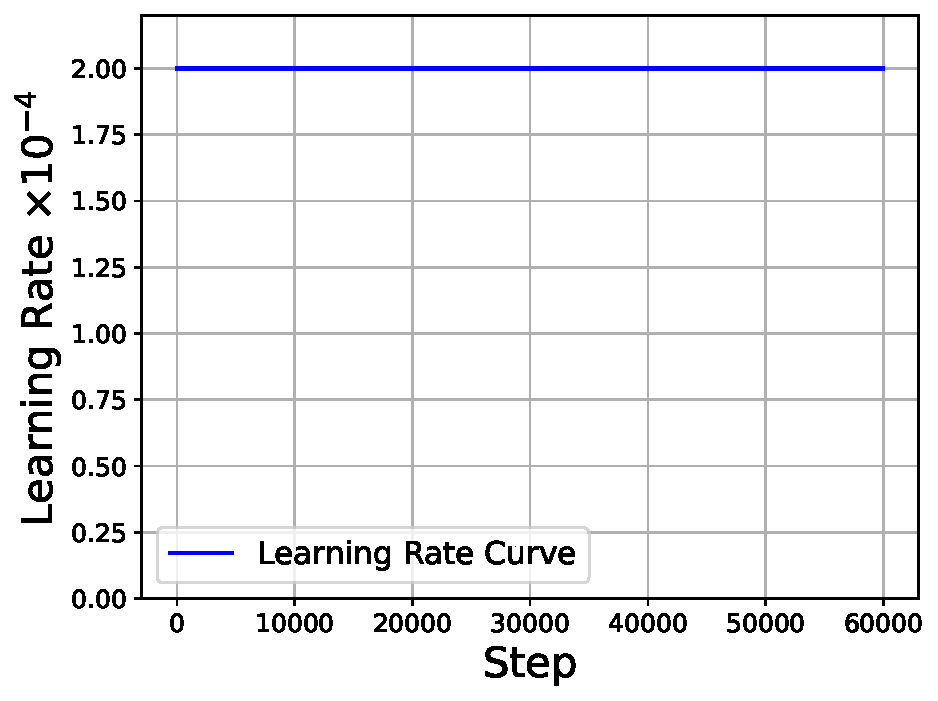
\includegraphics[width=0.32\textwidth]{images/pdfs_0.999_bigbig/lr_constant.pdf}
        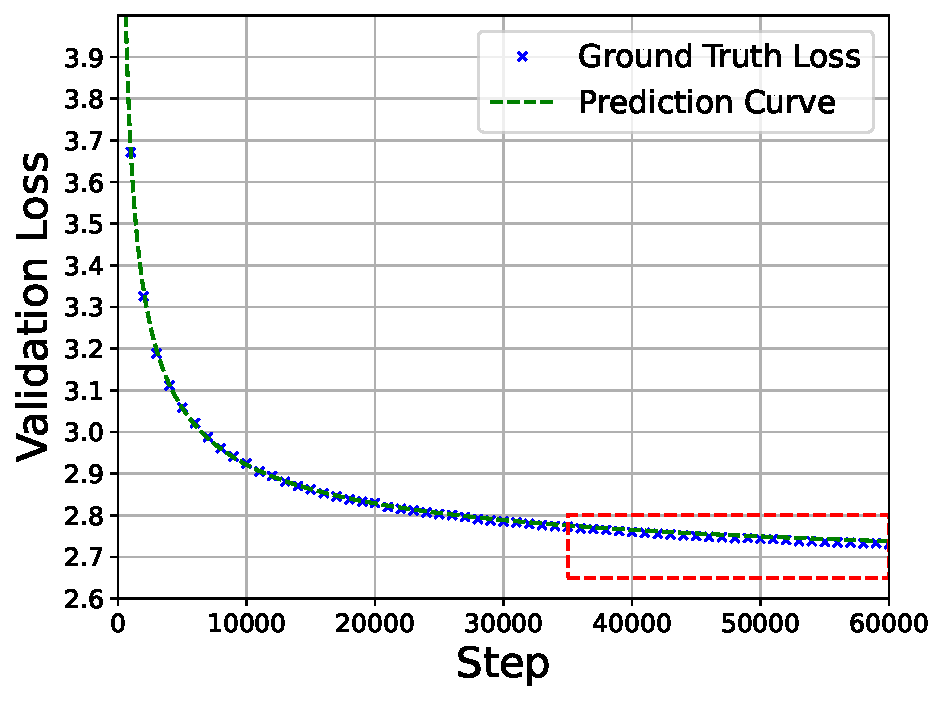
\includegraphics[width=0.32\textwidth]{images/pdfs_0.999_bigbig/predict_constant_zoomout.pdf}
        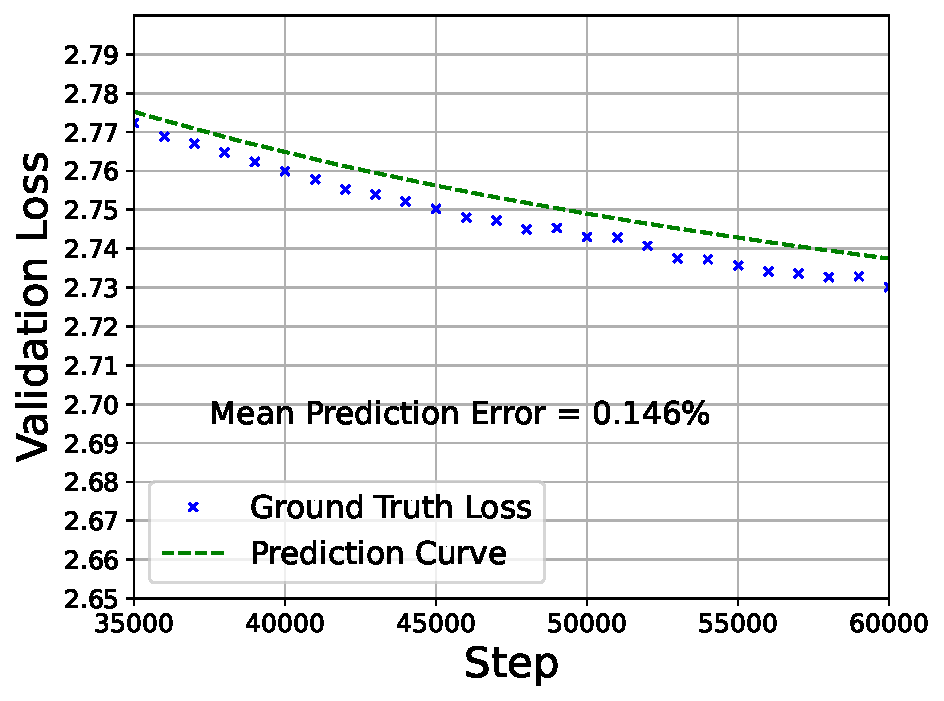
\includegraphics[width=0.32\textwidth]{images/pdfs_0.999_bigbig/predict_constant_zoomin.pdf}
        \caption{Full curve prediction of constant LRS.}
        \label{fig:prediction-constant}
    \end{subfigure}

    \begin{subfigure}[b]{\textwidth}
        \centering
        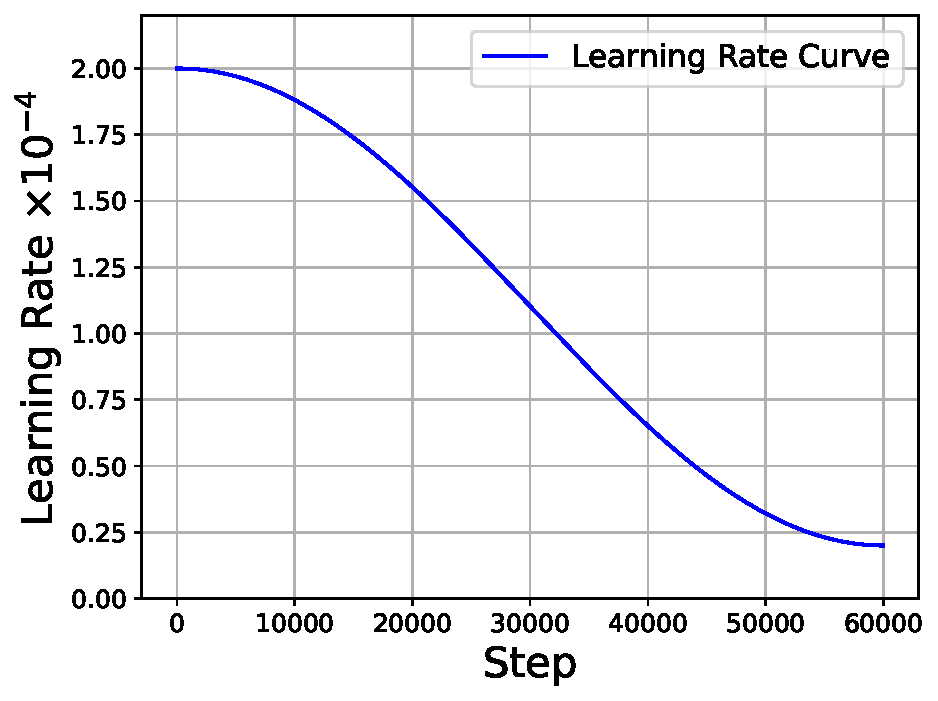
\includegraphics[width=0.32\textwidth]{images/pdfs_0.999_bigbig/lr_cosine.pdf}
        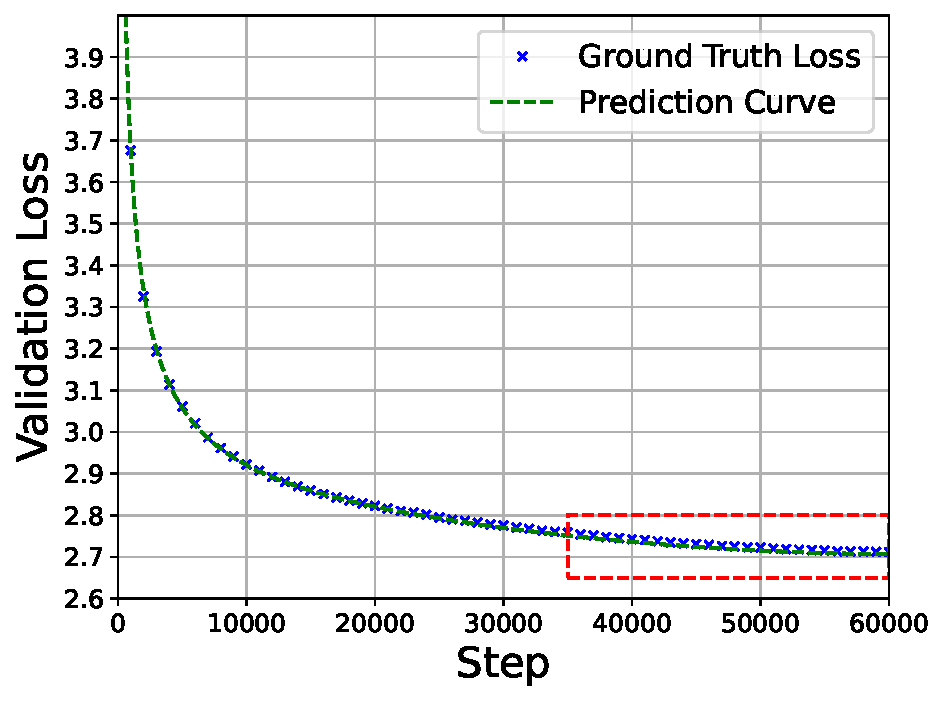
\includegraphics[width=0.32\textwidth]{images/pdfs_0.999_bigbig/predict_cosine_zoomout.pdf}
        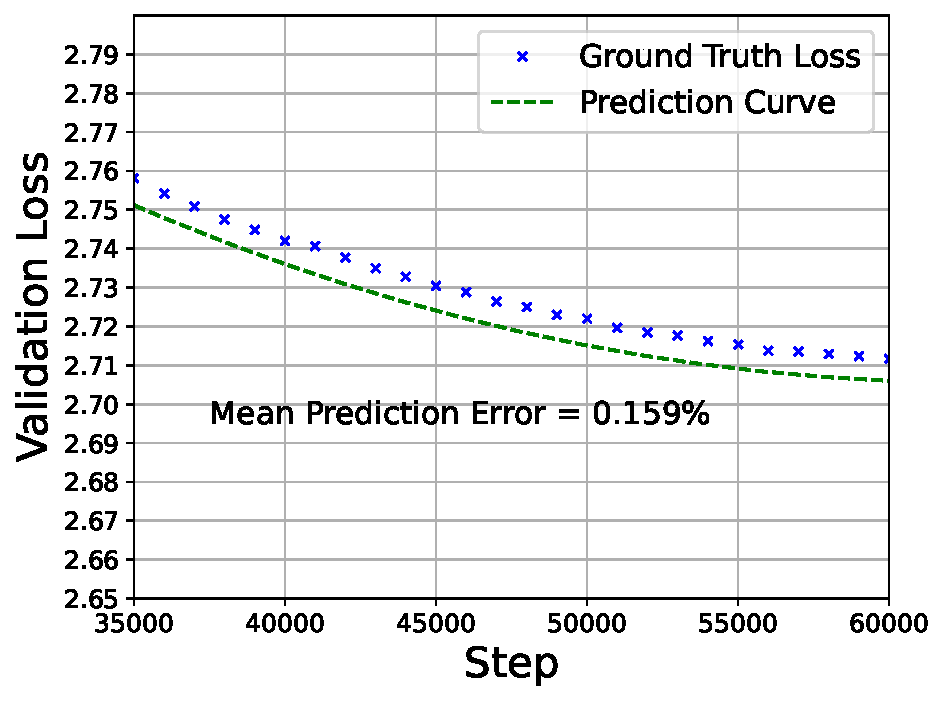
\includegraphics[width=0.32\textwidth]{images/pdfs_0.999_bigbig/predict_cosine_zoomin.pdf}
        \caption{Full loss curve prediction of the cosine LRS (60K steps, $\eta_{min} = 0.1\cdot\eta_{max}$).}
        \label{fig:prediction-cosine}
    \end{subfigure}

    \begin{subfigure}[b]{\textwidth}
        \centering
        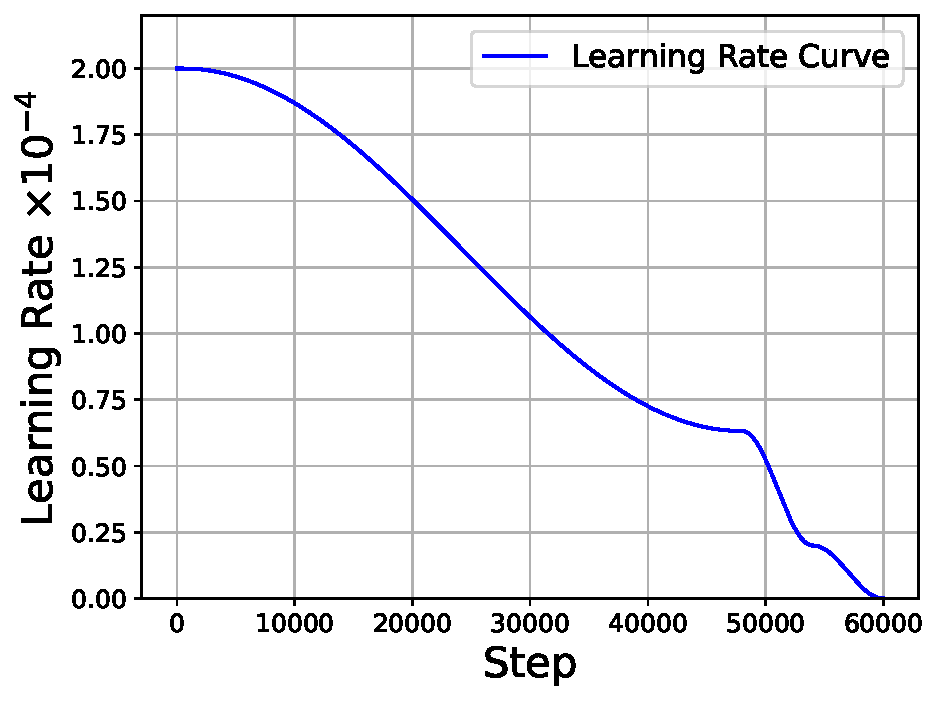
\includegraphics[width=0.32\textwidth]{images/pdfs_0.999_bigbig/lr_split-500-48000-0.316-54000-0.1-60000-0.0.pdf}
        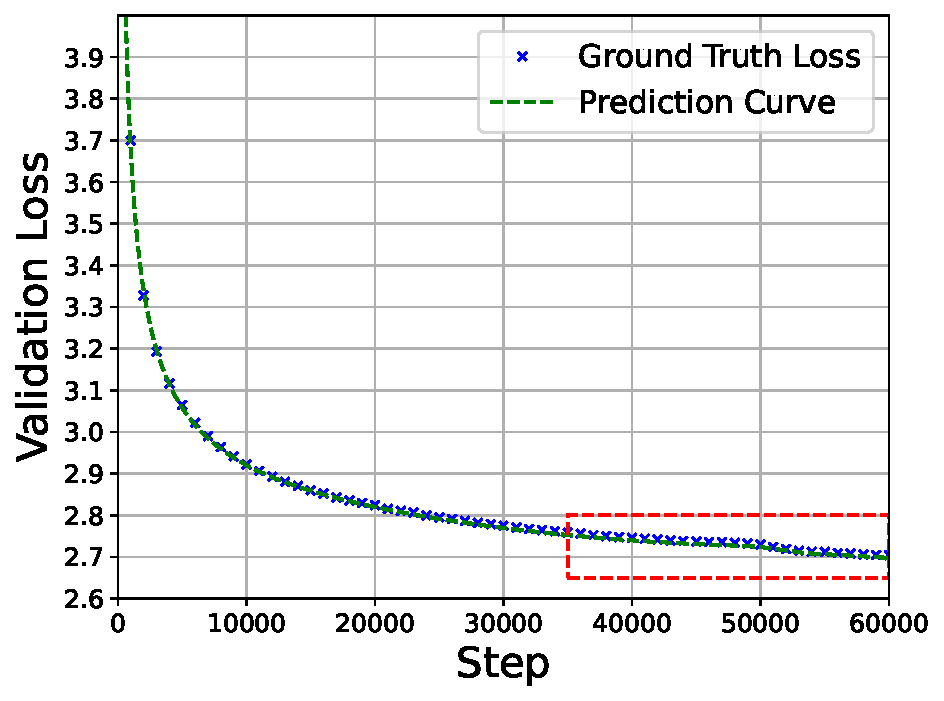
\includegraphics[width=0.32\textwidth]{images/pdfs_0.999_bigbig/predict_split-500-48000-0.316-54000-0.1-60000-0.0_zoomout.pdf}
        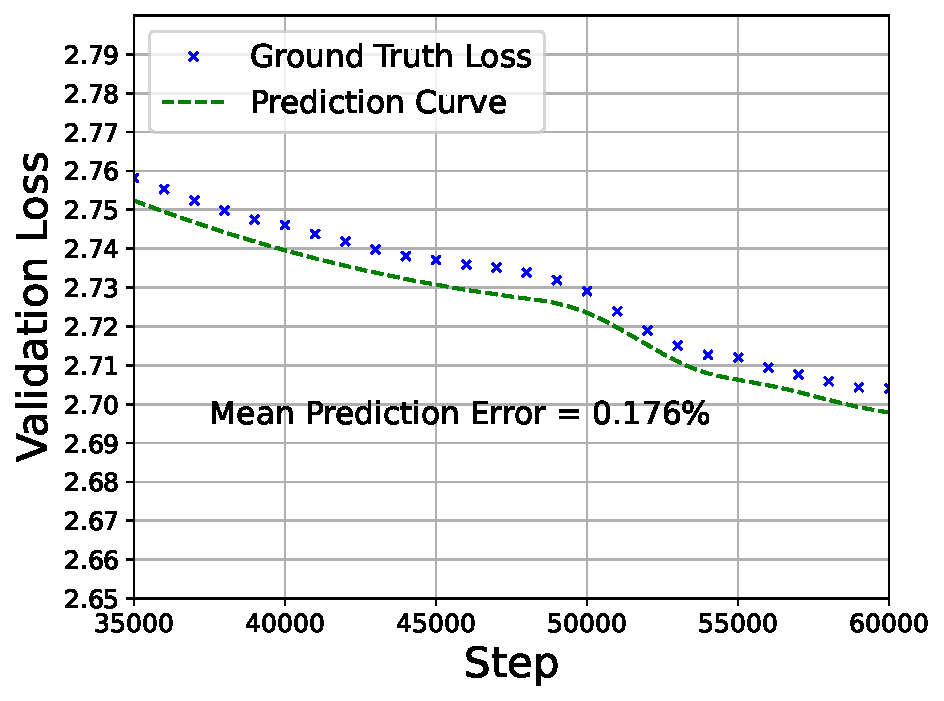
\includegraphics[width=0.32\textwidth]{images/pdfs_0.999_bigbig/predict_split-500-48000-0.316-54000-0.1-60000-0.0_zoomin.pdf}
        \caption{Full loss curve prediction of the multi-step cosine LRS (80\% + 10\% + 10\%)~\citep{deepseek-ai2024deepseek}.}
        \label{fig:prediction-multi-cosine}
    \end{subfigure}

    \begin{subfigure}[b]{\textwidth}
        \centering
        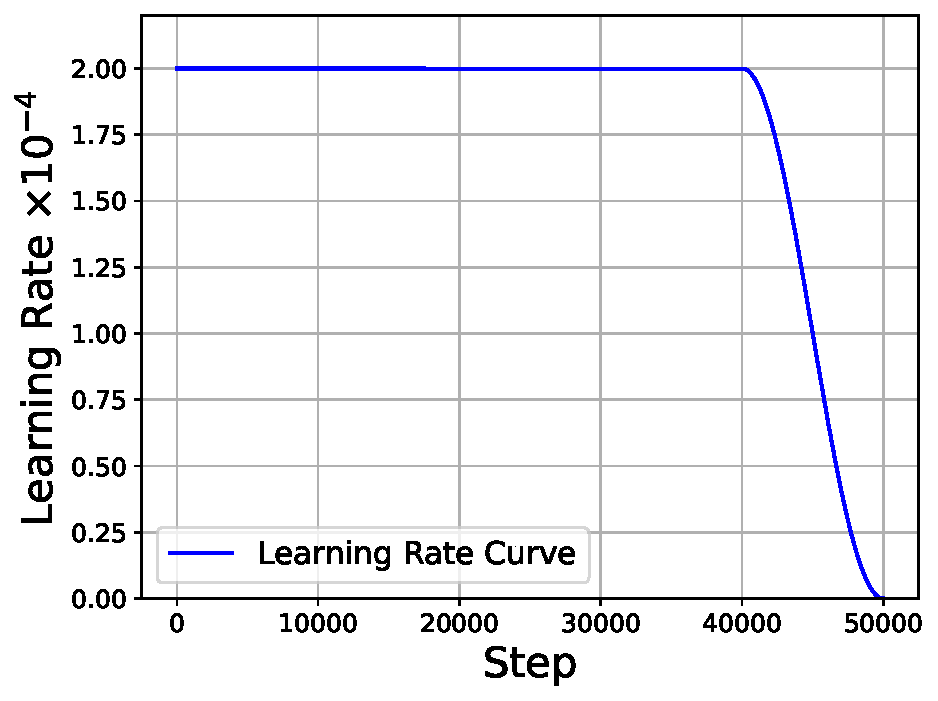
\includegraphics[width=0.32\textwidth]{images/pdfs_0.999_bigbig/lr_WSDW-40000-cosine-50000-cosine-60000.pdf}
        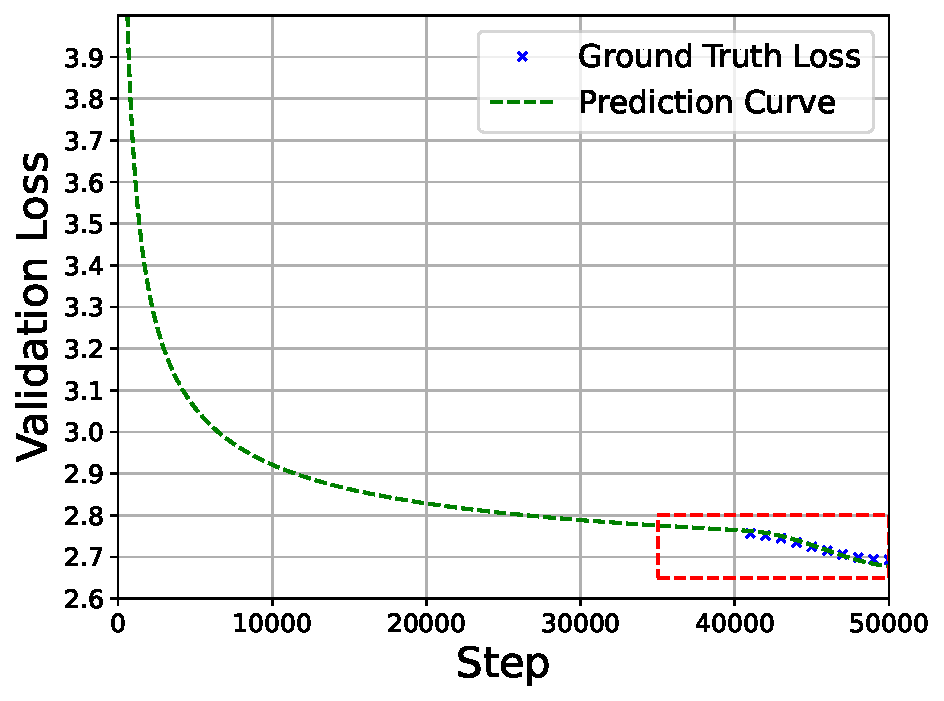
\includegraphics[width=0.32\textwidth]{images/pdfs_0.999_bigbig/predict_WSDW-40000-cosine-50000-cosine-60000_zoomout.pdf}
        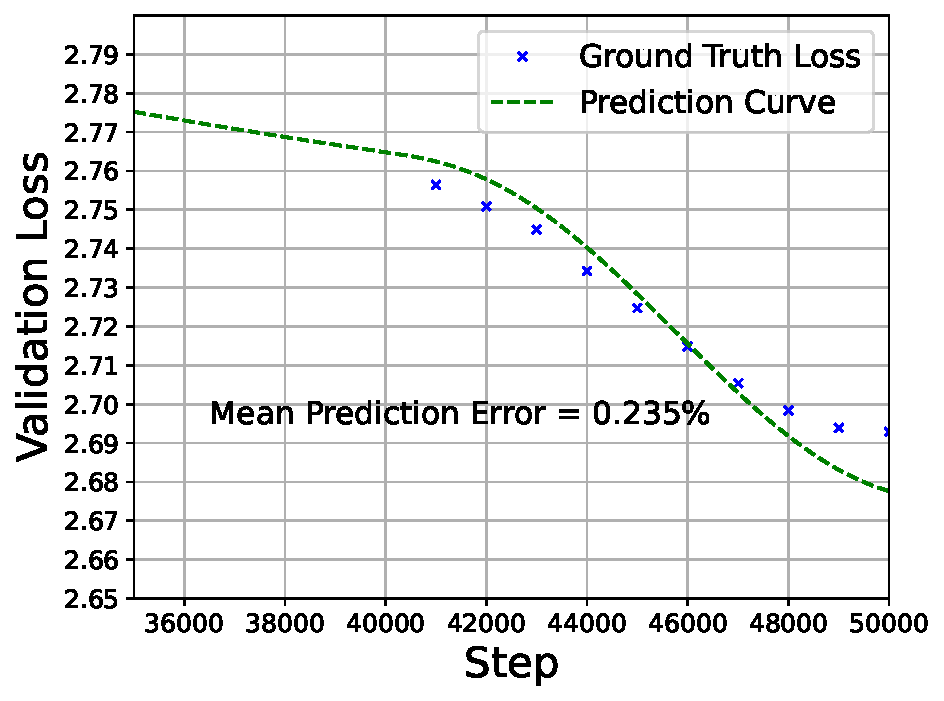
\includegraphics[width=0.32\textwidth]{images/pdfs_0.999_bigbig/predict_WSDW-40000-cosine-50000-cosine-60000_zoomin.pdf}
        \caption{Full Loss curve prediction of the WSD LRS (20\% cosine annealing to $\eta_{min} = 0$)~\citep{hu2024minicpm}.}
        \label{fig:prediction-wsd}
    \end{subfigure}
     \begin{subfigure}[b]{\textwidth}
        \centering
        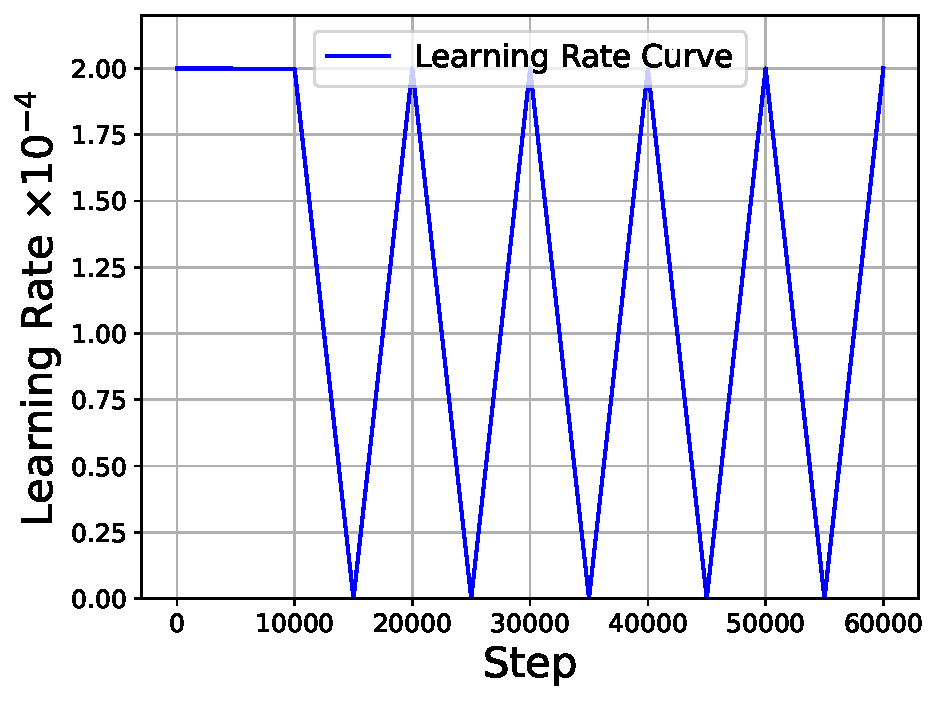
\includegraphics[width=0.32\textwidth]{images/plot_newxy/lr_all-10000-linear-5000-linear-5000.pdf}
        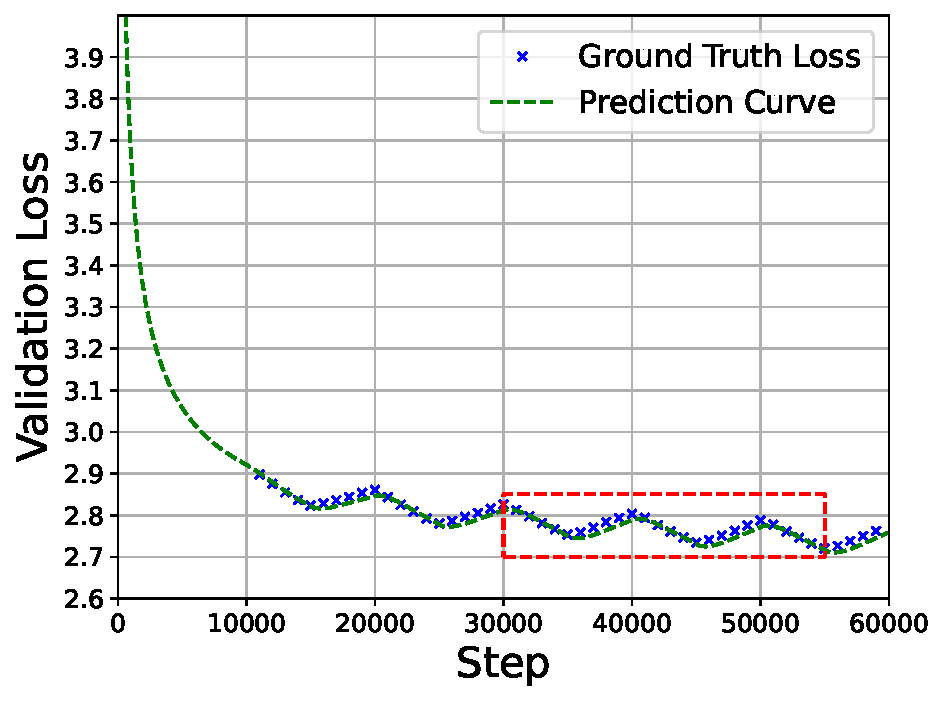
\includegraphics[width=0.32\textwidth]{images/plot_newxy/predict_all-10000-linear-5000-linear-5000_zoomout.pdf}
        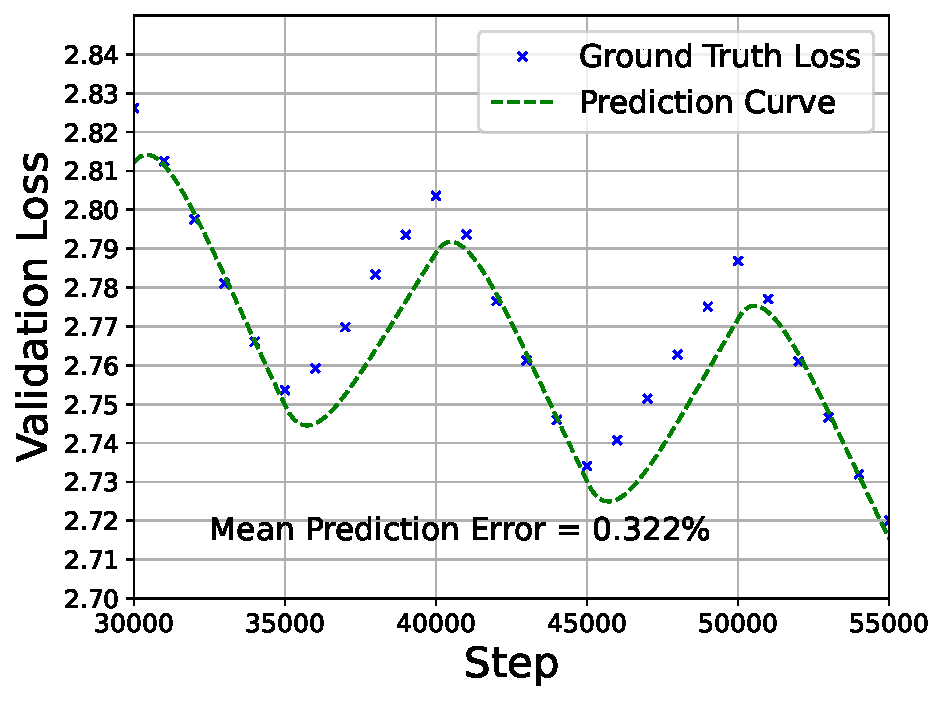
\includegraphics[width=0.32\textwidth]{images/plot_newxy/predict_all-10000-linear-5000-linear-5000_zoomin.pdf}
        \caption{Full Loss curve prediction of the Cyclic LRS \citep{smith2017cyclical} including multiple unseen LR re-warmup stages.}
        \label{fig:prediction-strange}
    \end{subfigure}
    
    \caption{Using the fitted equation from Fig.~\ref{fig:fit} to \textbf{predict} full loss curves for unseen LRS with 60K total steps. The left, middle, and right columns present the LR curve, the loss curve, and a zoomed-in view of loss curve, respectively. 
%     The red rectangle means the zoomed-in zone. 
    Warmup steps (500) are not shown in this figure.
    The fitted equation accurately predicts each loss curve, particularly for capturing the trend of loss changes as the LR varies. 
    Notable, all LRS and loss curves shown here were \textbf{unseen} during the fitting in Fig.~\ref{fig:fit}. The mean prediction errors across different LRS is as low as $\sim 0.2\%$.
    }
\label{fig:prediction}
\vspace{-10pt}
\end{figure}



We validate our proposed equation through extensive experiments and find that: (1) Our formulation performs consistently well across various hyper-parameters and model architectures;  (2) Eq.~\ref{eq:scaling} can be extended to incorporate other scaling factors, such as model sizes; (3) Our proposed equation accurately fits the loss curves of open-sourced models;
%(e.g. BLOOM~\citep{workshop2022bloom} and OLMo~\citep{groeneveld2024olmo}); 
(4) Our formulation can be used to verify and explain numerous previous findings regarding LR annealing and scheduling.

In Sec.~\ref{sec:theorem}, we derive the scaling law formulation with LR annealing and elucidate the potential theory underpinning our formulation. Extensive experiments are conducted to validate the formulation.
In Sec.~\ref{sec:takeaways}, we apply our formulation to verify and explain the empirical results from various previous studies. 
% These conclusions, which previously required substantial computational resources,
% can now be consolidated in a cost-free manner using our equation.
Our approach offers theoretical insights into the crux of loss drop, LR schedule, and LR annealing,
%(i.e., the art of balance between forward area and annealing area).
enabling LLM participants to better understand training dynamics of LLM and select optimal training recipes in advance.
In Sec.~\ref{sec:comparison}, we compare our approach to typical scaling law formula, such as the Chinchilla scaling law~\citep{hoffmann2022training}. We show that 
%chinchilla scaling law actually describes special cases (the endpoint of one full loss curve) of our equation, which means that 
our formulation is more general and requires significantly less compute (less than 1\%) to fit,
% Furthermore, we compare the computational costs required by the chinchilla scaling law and our equation, revealing that our equation offers significant savings in computational costs. 
which greatly democratizes the development of LLMs and scaling laws.
